\chapter{The discrete Fourier transform}
\label{chap-tfd}
\chapteroverview{The discrete Fourier transform turns cyclic structure into
computations on frequencies. Its fast algorithms make spectral methods practical
for signals, images, and convolution. We derive the main FFT factorizations,
explain their indexing and boundary conventions, and use the transform's
symmetries to construct eigenvectors and intermediate transforms.}

The DFT is the Fourier transform of a cyclic group, but its numerical use
raises additional questions: how should computations be factored, how are
samples stored, and what boundary conditions does a convolution impose?
The FFT is an algorithm for evaluating the DFT, not a different transform.
For historical context see Rockmore~\cite{rockmore-fft}; for algorithmic
background see Brigham~\cite{brigham-fft}, Arndt~\cite{arndt-algo-programmers},
and \emph{Numerical Recipes}~\cite{nr}. The Python implementations in
Section~\ref{sect1-listing-fft} accompany the derivations below.

\section{The language of signal processing}
\label{sect1-language-processing-signal}\label{notation-42}\index{Signal}
A sampled signal is a vector $f=(f[0],\ldots,f[N-1])\in\CC^N$.
It may come from a continuous signal $\wt f$ by $f[n]=\wt f(t_n)$.
For equally spaced samples on $[a,b)$,
$t_n=a+(b-a)n/N$, so the right endpoint is not sampled a second time.
The algebraic DFT is defined for every vector; interpreting its indices as
physical frequencies requires the sample spacing.

\begin{defn}[Discrete Fourier transform]
\label{notation-43}\index{Discrete Fourier transform}
Let $\omega_N=e^{2\pi\imath/N}$. The discrete Fourier transform (DFT) is
\begin{equation}
\label{eq-defn-tfd}
 \wh f[k]=\Ff(f)[k]=\sum_{n=0}^{N-1}f[n]\omega_N^{-nk},
 \qquad 0\leq k<N.
\end{equation}
Unless otherwise stated, $\Ff$ in this chapter denotes this unnormalized
negative-exponential transform on $\CC^N$.
\end{defn}
This is the convention used by NumPy's \texttt{fft}; its inverse includes
$1/N$. Replacing $\omega_N$ by another primitive root $\omega_N^r$,
with $\gcd(r,N)=1$, permutes the frequency labels by $k\mapsto rk\pmod N$.
It can also be interpreted as a change of generator of the cyclic group,
provided the signal coordinates are changed consistently.

\begin{rem}[Relation to the group Fourier transform]
For this chapter, index the characters by the negative exponential:
\begin{equation}
\label{eq-formula-character-znz}
 \chi_k(n)=\omega_N^{-kn},\qquad n\in\ZZ/N\ZZ.
\end{equation}
These are the inverses of the positively indexed cyclic characters in
Chapter~1. If $f_1:\ZZ/N\ZZ\to\CC$ is the function represented by $f$,
then $\wh f[k]=\wh{f_1}(\chi_k)$ under the group-transform convention
\eqref{eq-transf-fourier-grpe-abelien}. The transform itself is unchanged;
we have specified its frequency indexing.
\end{rem}

\begin{prop}[Inversion]
\label{prop-tfd-inverse}
For every $f\in\CC^N$,
\begin{equation}
\label{eq-transforme-fourier-discr-inverse}
 f[n]=\frac1N\sum_{k=0}^{N-1}\wh f[k]\omega_N^{nk},\qquad 0\leq n<N.
\end{equation}
\end{prop}
\begin{proof}
Substitute \eqref{eq-defn-tfd} and use
$\sum_{k=0}^{N-1}\omega_N^{k(n-m)}=N\delta_{nm}$ for $0\leq n,m<N$.
\end{proof}
\begin{cor}
The DFT is a linear isomorphism of $\CC^N$.
\end{cor}

\begin{prop}[Plancherel identity]
\label{prop-formula-floorel-tfd}
For $f,g\in\CC^N$,
\[
 \sum_{n=0}^{N-1}f[n]\ol{g[n]}
       =\frac1N\sum_{k=0}^{N-1}\wh f[k]\ol{\wh g[k]}.
\]
\end{prop}
Thus $N^{-1/2}\Ff$ is unitary, for either the usual or the normalized
discrete inner product. The factor in the unnormalized transform must be
retained when using it to transfer norms or orthonormal bases.

\section{Fast Fourier transforms}
\label{sect1-transform-fast}
An FFT evaluates the same finite sums as the DFT, rearranging their operations
to share intermediate results. We begin with power-of-two lengths and then
extend the factorization to general products. The derivations require only
complex arithmetic; the Good--Thomas exercise exposes the group-theoretic
structure behind one important variant.

\subsection{The radix-two algorithm}
\label{sect2-present-algo-fft}\index{FFT}\index{Divide and conquer}
Direct evaluation of
\begin{equation}
\label{eq-calcul-direct-tfd}
 \wh f[k]=\sum_{n=0}^{N-1}f[n]e^{-2\pi\imath kn/N}
\end{equation}
uses $N^2$ complex multiplications and $N(N-1)$ additions if every term is
counted, including trivial multiplications. This is $O(N^2)$ arithmetic.
For $N=2^p$, the radix-two Cooley--Tukey algorithm reduces it to
$O(N\log N)$ by repeatedly splitting the input into even and odd indices.

An inverse transform needs no fundamentally different algorithm:
\[
 \Ff^{-1}f=\frac1N\ol{\Ff(\ol f)}
          =\Ff(f_1),\qquad f_1[n]=\frac1Nf[(-n)\bmod N].
\]
Equivalently, reverse the sign of every exponential and divide once by $N$.
In particular, index zero stays fixed in the cyclic reversal.

For even $N$, split the sum according to input parity:
\begin{equation}
\label{eq-fft-dif}
 \wh f[k]=\sum_{n=0}^{N/2-1}f[2n]\omega_{N/2}^{-nk}
          +\omega_N^{-k}\sum_{n=0}^{N/2-1}f[2n+1]\omega_{N/2}^{-nk}.
\end{equation}
Define the even and odd subvectors
\begin{equation}
\label{eq-part-even-odd}
 f^0[n]=f[2n],\qquad f^1[n]=f[2n+1],\qquad 0\leq n<N/2.
\end{equation}
\label{notation-44}
Their DFTs have length $N/2$ and are periodic in $k$ with that period.
Using $\omega_N^{-(k+N/2)}=-\omega_N^{-k}$ gives
\begin{align}
\label{eq-danielson-lanczos-1}
 \wh f[k]&=\wh{f^0}[k]+\omega_N^{-k}\wh{f^1}[k],\\
\label{eq-danielson-lanczos-2}
 \wh f[k+N/2]&=\wh{f^0}[k]-\omega_N^{-k}\wh{f^1}[k],
 \qquad 0\leq k<N/2.
\end{align}
The same two shorter transforms therefore produce every output coefficient.

\begin{defn}[Halves and phase multiplication]
\label{notation-45}\label{notation-46}
For a vector $h$ of even length $N$, write $h_g$ and $h_d$ for its first
and second halves. In particular,
\begin{equation}
\label{eq-part-gd}
 \wh f_g[k]=\wh f[k],\qquad \wh f_d[k]=\wh f[k+N/2],\qquad 0\leq k<N/2.
\end{equation}
For $a\in\CC^M$ and $x\in\RR$, define the phase operator
\begin{equation}
\label{eq-operator-S}
 (\Ss_M^xa)[j]=e^{-2\pi\imath xj/M}a[j],\qquad 0\leq j<M.
\end{equation}
\end{defn}
The two recurrence equations become
\begin{align}
\label{eq-danielson-lanczos-a}
 \wh f_g&=\wh{f^0}+\Ss_{N/2}^{1/2}\wh{f^1},\\
\label{eq-danielson-lanczos-b}
 \wh f_d&=\wh{f^0}-\Ss_{N/2}^{1/2}\wh{f^1}.
\end{align}
They are often called the Danielson--Lanczos relations. This is
\emph{decimation in time} (DIT), because the input sample indices are split
by parity. Section~\ref{sect2-frequency-decimation} instead splits output
frequencies.

The elementary operation $(a,b)\mapsto(a+wb,a-wb)$ is a \emph{butterfly},
with $w=\omega_N^{-k}$ the \emph{twiddle factor}.
The crossing lines in Figure~\ref{fig-fft-butterfly-2points} indicate which
input contributes to each output. Figure~\ref{fig-fft-butterfly-8points}
shows the four butterflies that combine two length-four transforms.
\begin{figure}[tbp]
\centering
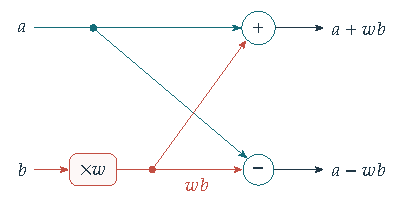
\includegraphics[width=.65\linewidth]{figures/chapter-discrete-fourier-transform/elementary-butterfly/figure.pdf}
\caption{An FFT butterfly: the same weighted value $wb$ enters the sum and the difference, with $w=\omega_N^{-k}$.}
\label{fig-fft-butterfly-2points}
\end{figure}
\begin{figure}[tbp]
\centering
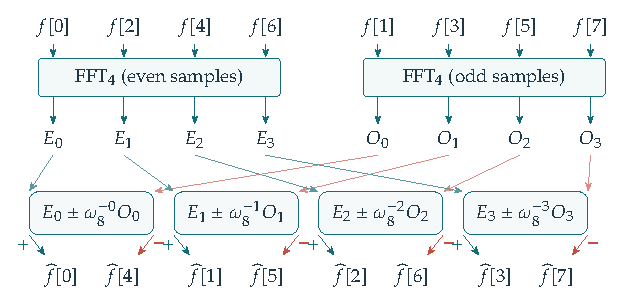
\includegraphics[width=1.0\linewidth]{figures/chapter-discrete-fourier-transform/eight-point-fft/figure.pdf}
\caption{The combination stage of an eight-point DIT FFT. Two four-point transforms produce $E_k$ and $O_k$; each butterfly combines $E_k$ with $\omega_8^{-k}O_k$.}
\label{fig-fft-butterfly-8points}
\end{figure}
A recursive implementation follows the equations directly. The function
\texttt{fft\_recursive} in Section~\ref{sect1-listing-fft} uses NumPy arrays
and an optional inverse flag; \texttt{phase\_multiply} implements $\Ss_M^x$.
The recursion is useful for understanding the factorization. Iterative
versions expose its memory layout more explicitly.

\subsection{Arithmetic cost}
\label{sect2-analyze-cost-fft}
\begin{prop}[FFT complexity]
If a combine stage costs $KN$ operations and a length-one transform costs
zero, the recurrence $C(N)=2C(N/2)+KN$ gives $C(N)=KN\log_2N$ for $N=2^p$.
More generally, an $O(N)$ combine stage gives $C(N)=O(N\log N)$.
\end{prop}
\begin{proof}
Set $D(p)=C(2^p)/2^p$. Then $D(p)=D(p-1)+K$ and $D(0)=0$.
Hence $D(p)=Kp$. Equivalently, each of the $p$ recursion levels costs $KN$.
\end{proof}
This arithmetic estimate explains the gain over direct evaluation.
Actual running time also depends on data movement, implementation, and
hardware; a count of complex operations alone does not determine it.

\subsection{Zero padding and other radices}
\label{sect2-variations-fft}
\begin{rem}[What zero padding changes]
Appending zeros to a length-$N$ vector and taking a length-$M$ DFT evaluates
the same trigonometric sum $\sum_{n=0}^{N-1}f[n]e^{-\imath n\theta}$ at
$\theta=2\pi k/M$. It does \emph{not} compute the original length-$N$ DFT
unless the required frequencies coincide. Padding is useful for denser
frequency sampling and for linear convolution. When the length-$N$ DFT
itself is required, use an algorithm for that length.
\end{rem}

\begin{rem}[Radix four and a general radix]
\label{rmk-radix-fft}\index{FFT!radix four}
A radix-$r$ split groups input indices by their residue modulo $r$.
For $N=rM$, set $f^b[n]=f[rn+b]$, for $0\leq b<r$ and $0\leq n<M$.
If $\sigma=1$ denotes the forward transform and $\sigma=-1$ the
unnormalized inverse, let $\wh{f^b}_{\sigma}$ use that same sign and set
$z_b[k]=\omega_N^{-\sigma bk}\wh{f^b}_{\sigma}[k]$.
Then
\[
 \wh f_{\sigma}[k+qM]=\sum_{b=0}^{r-1}\omega_r^{-\sigma bq}z_b[k],
 \qquad 0\leq k<M,\quad 0\leq q<r.
\]
Both the shorter transforms and the twiddle factors must change sign for
the inverse. Divide its final output by $N$.
For $r=4$, the four outputs at a fixed $k$ are
\[
\begin{array}{ll}
 z_0+z_1+z_2+z_3,&z_0-\imath\sigma z_1-z_2+\imath\sigma z_3,\\
 z_0-z_1+z_2-z_3,&z_0+\imath\sigma z_1-z_2-\imath\sigma z_3.
\end{array}
\]
Multiplication by $\pm1$ and $\pm\imath$ uses only sign changes and swaps
of real and imaginary parts. The split-radix method in
Exercise~\ref{exo-algo-split-radix} combines radix-two and radix-four splits.
\end{rem}

\subsection{The Cooley--Tukey factorization}
\label{sect2-transfo-cooley-tukey}
Suppose $N=pq$, without requiring $p$ and $q$ to be prime or coprime.
Starting again from
\begin{equation}
\label{eq-tfd-transfo-cooley-tukey}
 \wh f[k]=\sum_{n=0}^{N-1}f[n]\omega_N^{-nk},
\end{equation}
write $n=ap+b$ and $k=cq+d$, with
$0\leq a,d<q$ and $0\leq b,c<p$.
Both index maps are bijections by Euclidean division. Expanding the product,
\[
 (ap+b)(cq+d)=acN+adp+bcq+bd.
\]
The first term contributes a factor one. Define the length-$q$ vectors
$f_b[a]=f[ap+b]$. Then
\begin{equation}
\label{eqn-cooley-tukey-twiddle}
 \wh f[cq+d]=\sum_{b=0}^{p-1}\omega_p^{-bc}
                         \bigl(\omega_N^{-bd}\wh{f_b}[d]\bigr).
\end{equation}
This gives a concrete three-step algorithm: compute $p$ length-$q$ DFTs,
multiply their entries by the twiddle factors $\omega_N^{-bd}$, and compute
$q$ length-$p$ DFTs. The input array $(f[ap+b])_{a,b}$ has $q$ rows and
$p$ columns; specifying this orientation avoids ambiguous reshaping.
With direct shorter transforms, the cost is $O(pq(p+q))$.
Recursing through $N=p_1\cdots p_s$ gives $O(N\sum_jp_j)$ operations.
Bounded factors therefore give $O(N\log N)$, while a large prime factor
calls for another method. Good--Thomas removes twiddle factors for coprime
factors (Exercise~\ref{exo-algo-good-thomas}); chirp methods offer another
route for lengths with inconvenient factorizations.

\subsection{Bit reversal and iterative implementation}
\label{sect2-impl-concrete}\index{Bit reversal}
The recursive DIT algorithm splits even and odd indices at every level.
For $N=2^p$, following these choices down the recursion tree reads the bits
of an input index from least to most significant. The resulting leaf order
is therefore the bit-reversal permutation
\[
 n_p(i)=\sum_{t=0}^{p-1}i_t2^{p-1-t},
 \qquad i=\sum_{t=0}^{p-1}i_t2^t.
\]
For example, $n_3(6)=n_3((110)_2)=(011)_2=3$.
It is an involution. If $B_pf$ denotes the permuted vector
$(B_pf)[i]=f[n_p(i)]$, then
\[
 B_pf=\bigl(B_{p-1}f^0,\ B_{p-1}f^1\bigr).
\]
After this initial permutation, successive stages combine contiguous blocks
of lengths $2,4,\ldots,N$. The butterfly recurrence is still
\begin{equation}
\label{eq-rec-relation-fft}
 \wh f[k]=\wh{f^0}[k]+\omega_N^{-k}\wh{f^1}[k]
 \quad(0\leq k<N/2),
\end{equation}
with the corresponding minus sign for the second half. We are changing
storage order, not taking the DFT of the permuted signal as a new input.

Program~\ref{listing-rev_bits} generates the permutation in $O(N)$ arithmetic
and index operations by the recursion of Exercise~\ref{exo-bit-reversal}.
An iterative DIT transform can then overwrite its working array stage by
stage. The Python implementation copies the input and uses temporary arrays
for each butterfly block; it does not claim the strict constant-workspace
behavior of a low-level scalar implementation.
\begin{figure}[tbp]
\centering
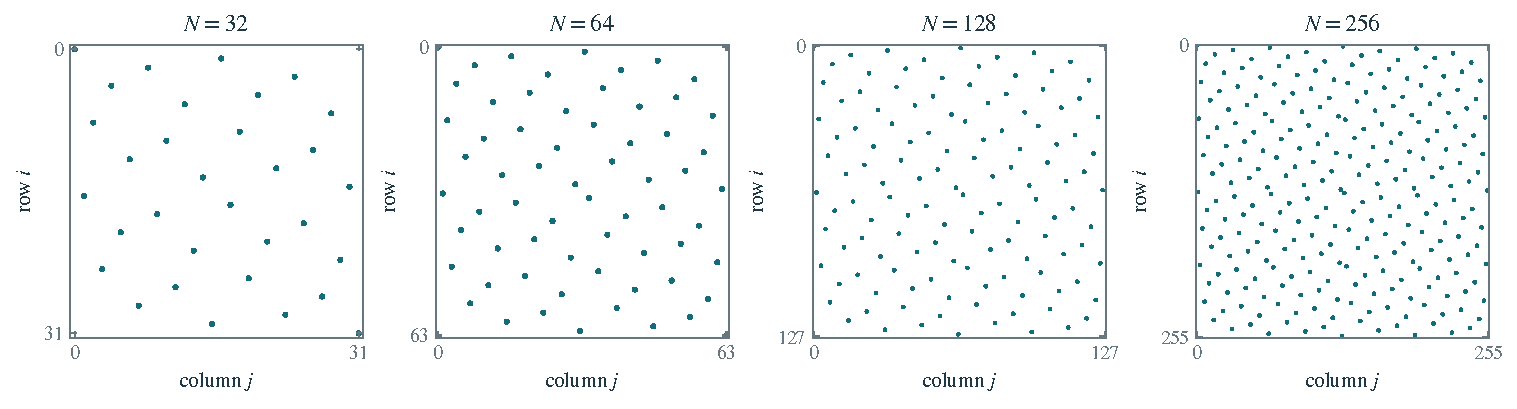
\includegraphics[width=1.0\linewidth]{figures/chapter-discrete-fourier-transform/bit-reversal-matrices/figure.pdf}
\caption{Bit-reversal permutation matrices for $N=32,64,128,256$. A dot in row $i$ and column $j$ means that the bits of $j$ are those of $i$ in reverse order.}
\label{fig-rev-bit-matrix}
\end{figure}
\begin{figure}[tbp]
\centering
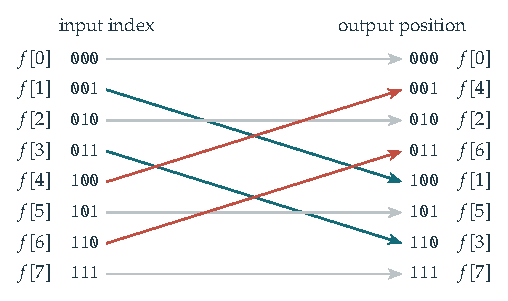
\includegraphics[width=.65\linewidth]{figures/chapter-discrete-fourier-transform/bit-reversal-permutation/figure.pdf}
\caption{Bit reversal on eight entries. The binary labels make the swaps $1\leftrightarrow4$ and $3\leftrightarrow6$ explicit; the other four indices are fixed.}
\label{fig-inversion-bits}
\end{figure}

\subsection{Decimation in frequency}
\label{sect2-frequency-decimation}\index{Decimation!frequency}
DIF splits the output indices by parity. Write $f_g[n]=f[n]$ and
$f_d[n]=f[n+N/2]$ for $0\leq n<N/2$. Then
\[
 \wh f[k]=\sum_{n=0}^{N/2-1}\bigl(f_g[n]+(-1)^kf_d[n]\bigr)\omega_N^{-nk}.
\]
For $0\leq k<N/2$, the even and odd outputs are
\begin{align*}
 \wh f[2k]&=\sum_{n=0}^{N/2-1}(f_g[n]+f_d[n])\omega_{N/2}^{-nk},\\
 \wh f[2k+1]&=\sum_{n=0}^{N/2-1}\omega_N^{-n}
                          (f_g[n]-f_d[n])\omega_{N/2}^{-nk}.
\end{align*}
In the notation of \eqref{eq-operator-S},
\[
 (\wh f)^0=\Ff(f_g+f_d),\qquad
 (\wh f)^1=\Ff\bigl(\Ss_{N/2}^{1/2}(f_g-f_d)\bigr).
\]
The phase in the odd branch depends on the input summation index $n$.
Also, $(\wh f)^0$ denotes the even entries of the output, whereas
$\wh{f^0}$ denotes the transform of the even input entries; these differ.

An iterative DIF implementation combines blocks of lengths $N,N/2,\ldots,2$.
Starting with naturally ordered data, it leaves its outputs in bit-reversed
order. Applying $B_p$ at the end restores natural frequency order.
Program~\ref{listing-fft_dif} follows this convention.
DIT and DIF express dual factorizations: DIT permutes the input first, while
DIF permutes the output last. Their practical performance depends on the
implementation and the data layout, not solely on this distinction.
For broader surveys see Burrus~\cite{burrus-fft}.

\subsection{Matrix form}
\label{sect1-matrix-writing}\index{Fourier matrix}\index{Vandermonde matrix}
The matrix of the DFT is
\begin{equation}
\label{eq-defn-matrix-fourier}
 \Omega_N=(\omega_N^{-kn})_{0\leq k,n<N}.
\end{equation}
It is a symmetric Vandermonde matrix. Applied to polynomial coefficients,
it evaluates the unique polynomial of degree \emph{at most} $N-1$ at the
$N$ distinct nodes $1,\omega_N^{-1},\ldots,\omega_N^{-(N-1)}$.
Section~\ref{sect1-calculations-products} uses this connection for polynomial
multiplication and interpolation.

\label{notation-47}
Writing $A^*=\ol A^{\mathsf T}$ for the adjoint,
$\Omega_N^{-1}=N^{-1}\Omega_N^*$ and $\Omega_N\Omega_N^*=NI_N$.
Thus $U_N=\Omega_N/\sqrt N$ is unitary. The matrix is symmetric but
in general is \emph{not} Hermitian.
If $P_{\rm eo}f=(f^0,f^1)$ and
$\Delta=\operatorname{diag}(1,\omega_N^{-1},\ldots,\omega_N^{-(N/2-1)})$,
then the radix-two factorization is
\[
 \Omega_N=
 \begin{pmatrix}I&\Delta\\I&-\Delta\end{pmatrix}
 \begin{pmatrix}\Omega_{N/2}&0\\0&\Omega_{N/2}\end{pmatrix}P_{\rm eo}.
\]
The permutation is part of the factorization and cannot be omitted.

\section{Circular and linear convolution}
\label{sect1-tfd-prod-convol}
The convolution theorem of Chapter~1 becomes an efficient algorithm on
sampled signals. Its interpretation depends on whether indices wrap around
or signals are extended by zero.

\subsection{Circular convolution}
\label{sect1-convolution-circular}
\begin{defn}[Circular convolution]
For $f,g\in\CC^N$, define
\begin{equation}
\label{eq-convolution-discrete}
 (f*g)[n]=\sum_{k=0}^{N-1}f[k]g[(n-k)\bmod N],\qquad 0\leq n<N.
\end{equation}
\end{defn}
This is convolution on $\ZZ/N\ZZ$. It is bilinear, associative, and
commutative, with unit $\delta_0$. These properties follow from the group
algebra, or directly by changing summation indices. Without modulo notation,
\[
 (f*g)[n]=\sum_{k=0}^nf[k]g[n-k]
             +\sum_{k=n+1}^{N-1}f[k]g[n-k+N].
\]
Both sums contain a difference of indices, not a product.

\begin{prop}[DFT convolution theorem]
\label{prop-convol-tfd}
For two length-$N$ vectors,
\begin{equation}
\label{eq-formula-convolution-tfd}
 \wh{f*g}[k]=\wh f[k]\wh g[k],\qquad 0\leq k<N.
\end{equation}
\end{prop}
\begin{proof}
As functions $f_1,g_1$ on the cyclic group,
\begin{equation}
\label{eq-lien-tfd-trans-fourier}
 \wh f[k]=\wh{f_1}(\chi_k),\qquad \wh g[k]=\wh{g_1}(\chi_k).
\end{equation}
The group convolution theorem gives the result.
Alternatively, set $m=n-j$ modulo $N$ in the double sum for
$\wh{f*g}[k]$; the factor $\omega_N^{-k(m+j)}$ separates into a product,
leaving the two Fourier sums.
\end{proof}
Circular convolution treats a finite vector as one period of a signal.
This is a boundary model; it need not agree with extending the signal by zero.

\subsection{Computing convolution with an FFT}
\label{sect1-convolution-calcul-fft}
The theorem and inversion give
\[
 f*g=\Ff^{-1}(\wh f\cdot\wh g).
\]
Two forward FFTs, $N$ pointwise multiplications, and an inverse FFT cost
$O(N\log N)$, compared with $O(N^2)$ for direct convolution.
If one filter is fixed, its transform can be reused.
For a very short filter, direct convolution may still be preferable because
it avoids the overhead of the transforms.

\subsection{Linear convolution and zero padding}
\label{sect1-convolution-acyclic}\index{Convolution!linear}
For finitely supported sequences $f_1,f_2:\ZZ\to\CC$, define
\begin{equation}
\label{eq-convolution-acyclic}
 (f_1\star f_2)[n]=\sum_{k\in\ZZ}f_1[k]f_2[n-k].
\end{equation}
This is \emph{linear} or \emph{acyclic} convolution. Its support satisfies
$\Supp(f_1\star f_2)\subset\Supp(f_1)+\Supp(f_2)$.
If the input supports are contained in intervals of lengths $N_1$ and $N_2$,
the output is contained in an interval of length $N_1+N_2-1$.
These are interval lengths, not the numbers of nonzero entries in sparse supports.

Suppose first that the intervals start at zero. Pad both vectors with zeros
to a common length $L\geq N_1+N_2-1$. Their length-$L$ circular convolution
agrees with their linear convolution on $0,\ldots,N_1+N_2-2$, and is zero
at the remaining indices. Indeed, no two potentially nonzero output indices
are congruent modulo $L$. This is the condition that prevents wrap-around.
An FFT at a convenient such length computes the linear convolution exactly
in exact arithmetic; padding introduces no approximation here.

For a kernel supported on $\{-P,\ldots,Q\}$, store each coefficient at its
residue modulo $L$: positive indices at the beginning and negative indices
at the end. With $f_1$ supported on $0,\ldots,N_1-1$ and
$L\geq N_1+P+Q$, the output support is contained in
$\{-P,\ldots,N_1-1+Q\}$, and
\[
 (f_1\star f_2)[n]=(\wt f_1*\wt f_2)[n\bmod L]
 \quad\text{throughout this interval}.
\]
In particular, negative output indices occupy the final slots. One must not
append padding after a negative-index tail without moving that tail to the
end of the new array.

Figure~\ref{fig-diff-conv-linear-circular} compares periodic and zero boundary
conditions for a short averaging filter. Their interior outputs agree where
the whole filter support remains inside the sample interval. Near an edge,
periodic convolution draws values from the opposite edge, while zero extension
reduces the average. The appropriate boundary model depends on the application;
zero extension is not inherently free of boundary artifacts.
\begin{figure}[tbp]
\centering
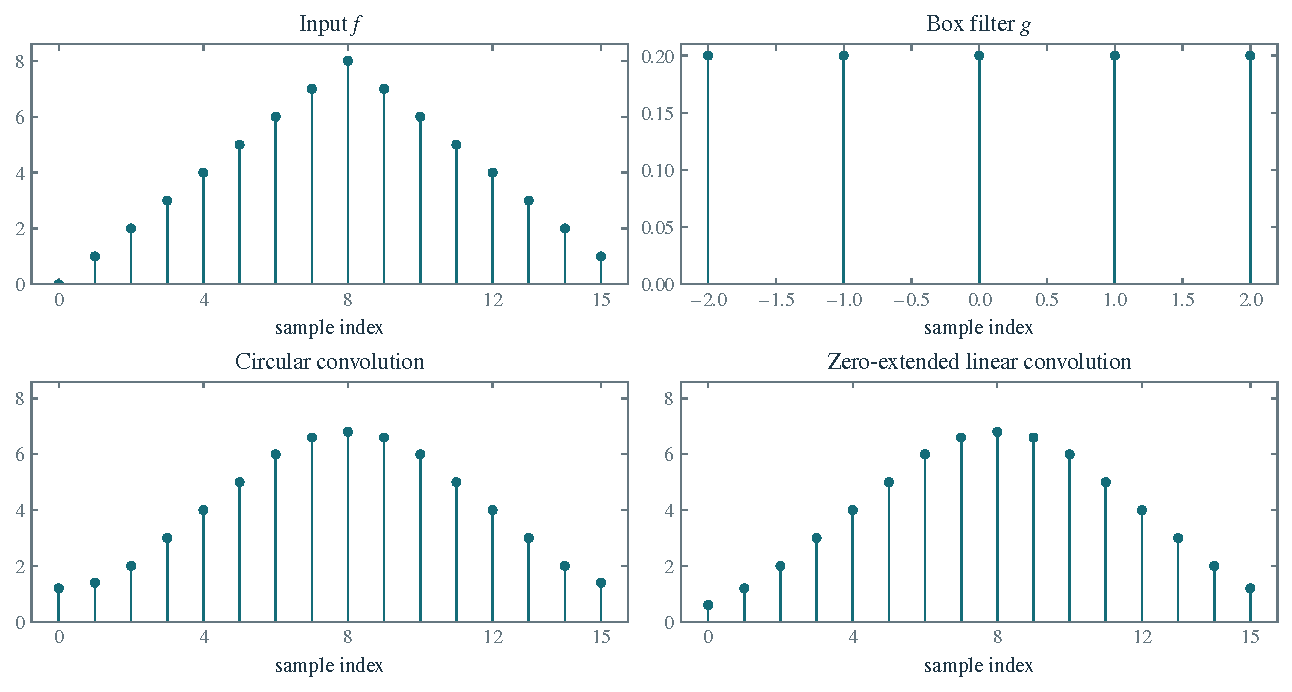
\includegraphics[width=1.0\linewidth]{figures/chapter-discrete-fourier-transform/linear-and-circular-convolution/figure.pdf}
\caption{Circular and zero-extended linear convolution of a triangular signal with a unit-sum five-tap box filter. The outputs agree away from the endpoints.}
\label{fig-diff-conv-linear-circular}
\end{figure}
Exercise~\ref{exo-calcul-convolution-fft} develops overlap-add convolution
for a long signal and a short filter. Chapter~\ref{chap-applications-tfd}
uses these operations for filtering.

\section{Higher-dimensional transforms}
\label{sect1-tfd-dim-sup}
A rectangular array corresponds to a function on a product of cyclic groups.
The characters factor by coordinate, so both the formulas and the algorithms
separate into one-dimensional transforms.

\subsection{The two-dimensional DFT}
\label{sect2-transforme-discrete-2d}
\begin{defn}[Two-dimensional DFT]
For $f\in\CC^{N\times P}$, define
\begin{equation}
\label{eq-defn-tfd-2d}
 \wh f[k,l]=\sum_{i=0}^{N-1}\sum_{j=0}^{P-1}
                       f[i,j]\omega_N^{-ik}\omega_P^{-jl}.
\end{equation}
Here $0\leq k<N$ and $0\leq l<P$.
\end{defn}
The characters of $\ZZ/N\ZZ\times\ZZ/P\ZZ$ are
$\chi_{k,l}(i,j)=\omega_N^{-ik}\omega_P^{-jl}$, so the formula is the
corresponding group Fourier transform.

\begin{prop}[Two-dimensional inversion]
For $0\leq i<N$ and $0\leq j<P$,
\[
 f[i,j]=\frac1{NP}\sum_{k=0}^{N-1}\sum_{l=0}^{P-1}
                             \wh f[k,l]\omega_N^{ik}\omega_P^{jl}.
\]
\end{prop}
The proof applies character orthogonality along each coordinate.
To compute the forward transform, first transform every row, then every
column of the result. The order of these two passes can be reversed.
In matrix form,
\[
 \wh f=\Omega_Nf\Omega_P^{\mathsf T}=\Omega_Nf\Omega_P,
\]
because the Fourier matrices are symmetric. The cost is
$O(NP(\log N+\log P))$. The same separation works in any dimension.

Figure~\ref{fig-tfd-2d} displays an image and the magnitude of its spectrum,
with zero frequency shifted to the center for readability.
For signed frequency indices $(k,l)$ and unit pixel spacing, the frequency
vector is $(k/N,l/P)$; its Euclidean norm is the spatial frequency, and it
points in the direction of variation, normal to the stripes of a plane wave.
The complex coefficient also carries phase, which a magnitude display omits.
\begin{figure}[tbp]
\centering
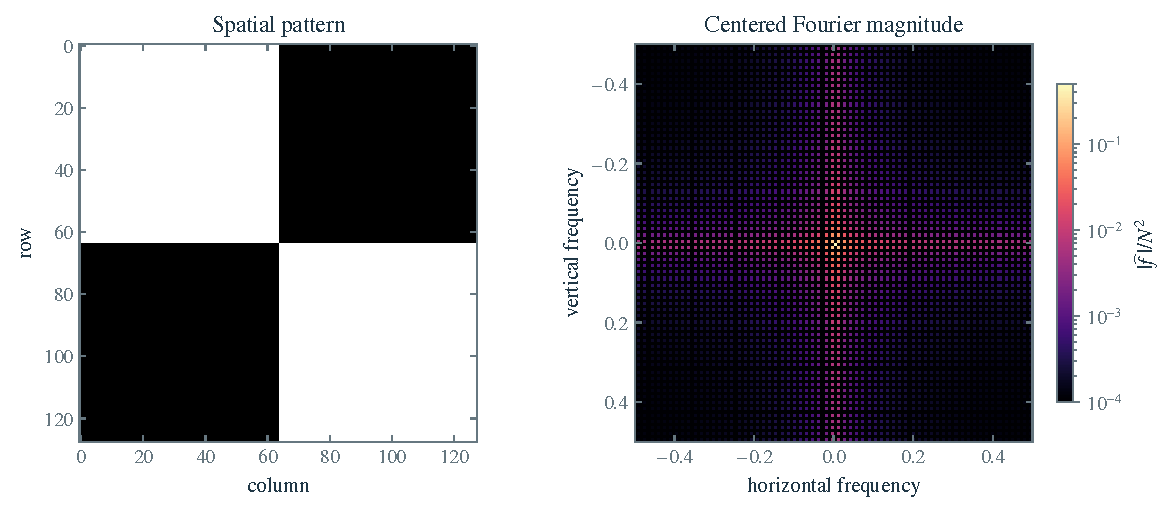
\includegraphics[width=1.0\linewidth]{figures/chapter-discrete-fourier-transform/two-dimensional-dft/figure.pdf}
\caption{A two-dimensional checker pattern and its centered Fourier magnitude. The logarithmic color scale reveals the weaker frequencies.}
\label{fig-tfd-2d}
\end{figure}

\subsection{Two-dimensional convolution}
\label{sect2-convolution-2d}
\begin{defn}[Circular convolution of arrays]
For $f,g\in\CC^{N\times P}$,
\begin{equation}
\label{eq-defn-product-convol-2d}
 (f*g)[i,j]=\sum_{k=0}^{N-1}\sum_{l=0}^{P-1}
                       f[k,l]g[(i-k)\bmod N,(j-l)\bmod P].
\end{equation}
\end{defn}
This uses periodic boundaries along both axes.
\begin{prop}[Two-dimensional convolution theorem]
\label{prop-convol-tfd-2d}
\begin{equation}
\label{eq-formula-convolution-tfd-2d}
 \wh{f*g}[k,l]=\wh f[k,l]\wh g[k,l].
\end{equation}
\end{prop}
\begin{proof}
Apply the group convolution theorem to $\ZZ/N\ZZ\times\ZZ/P\ZZ$,
or separate the exponential after substituting the two difference indices.
\end{proof}
Two forward FFTs, a pointwise product, and an inverse FFT therefore compute
the convolution. For linear convolution of arrays, pad along each axis to
at least the sum of the two side lengths minus one. A centered kernel's origin
must be moved to index $(0,0)$ in the padded array before transformation.

Convolution with a nonnegative kernel whose \emph{discrete sum} is one forms
a weighted average. Figure~\ref{fig-convolution-2d} illustrates the smoothing
of an irregular surface. Its continuum analogue uses a kernel of integral one;
the discrete formula uses a sum, without an implicit grid-spacing factor.
\begin{figure}[tbp]
\centering
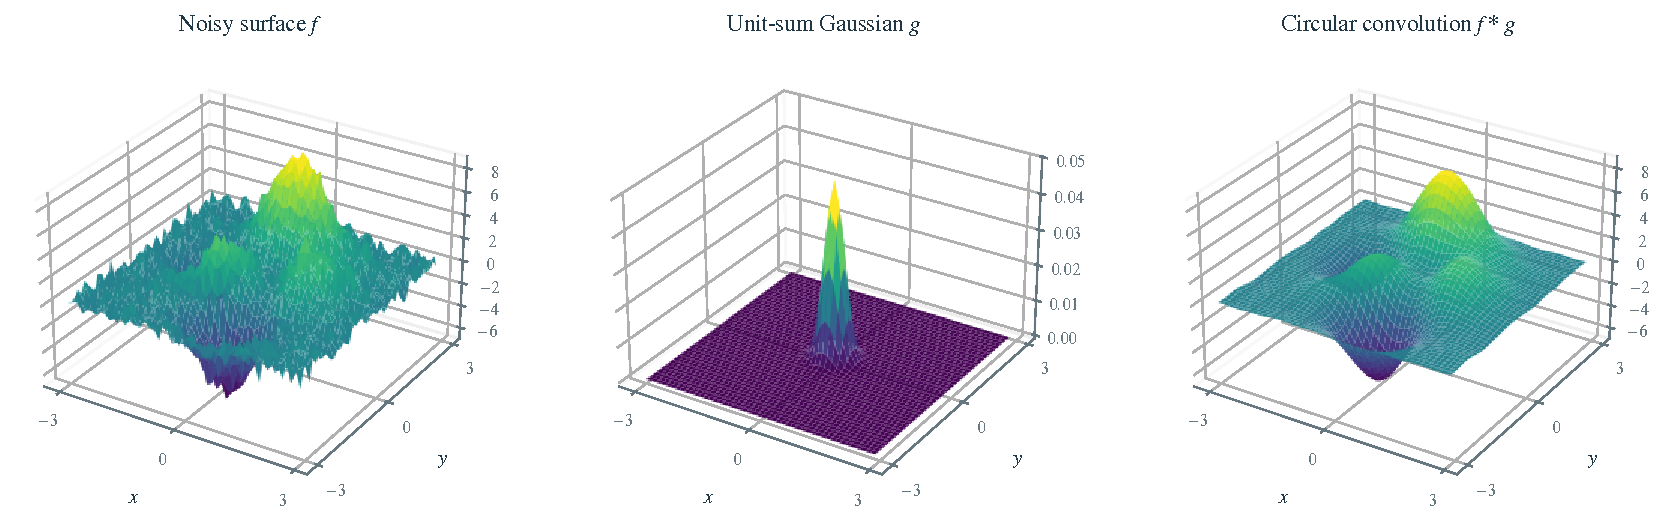
\includegraphics[width=1.0\linewidth]{figures/chapter-discrete-fourier-transform/two-dimensional-convolution/figure.pdf}
\caption{Circular Gaussian smoothing of a noisy surface. The discrete kernel has unit sum; its center is shifted to index $(0,0)$ before the FFT.}
\label{fig-convolution-2d}
\end{figure}

\section{Symmetry and spectral structure}
\label{sect1-symetrie-tfd}
The fourth power of a normalized DFT is the identity. This simple relation
restricts its spectrum and gives explicit projections onto its eigenspaces.
It also reveals the choices involved in defining fractional powers.

\subsection{Symmetry identities}
\label{sect2-prop-symmetry}
\begin{defn}[Cyclic reversal]
\label{defn-symmetry-operator}\label{notation-48}
For $f\in\CC^N$, define
\begin{equation}
\label{eq-defn-symmetrical-sample}
 f^\sharp[n]=f[(-n)\bmod N].
\end{equation}
Thus $f^\sharp=(f[0],f[N-1],\ldots,f[1])$.
A vector is symmetric if $f^\sharp=f$ and antisymmetric if $f^\sharp=-f$.
\end{defn}
\begin{defn}[Symmetric and antisymmetric parts]
\label{defn-parts-sym-anti-sym}\label{notation-49}
Set $\psym f=(f+f^\sharp)/2$ and $\pasym f=(f-f^\sharp)/2$.
Then $f=\psym f+\pasym f$ is an orthogonal decomposition.
\end{defn}

\begin{prop}[Symmetry of the DFT]
For every $f\in\CC^N$,
\[
 \Ff(f^\sharp)=(\Ff f)^\sharp=N\Ff^{-1}f,
 \qquad \Ff^2f=Nf^\sharp,
 \qquad \Ff(\ol f)=\ol{(\Ff f)^\sharp}.
\]
Consequently, the DFT preserves the symmetric and antisymmetric subspaces.
For real symmetric input its output is real; for real antisymmetric input
its output is purely imaginary.
\end{prop}
\begin{proof}
Substitute $m=-n$ modulo $N$ in the Fourier sum for $f^\sharp$ to reverse
the exponential's sign. Applying inversion gives the first two identities.
Conjugating the Fourier sum gives the third. If $f$ is real, this last
identity states that $\wh f[-k]=\ol{\wh f[k]}$; combining it with symmetry
or antisymmetry proves the final claims.
\end{proof}

\subsection{Eigenvectors and fractional powers}
\label{sect2-eigenvalues-tfd}
Write $U=N^{-1/2}\Ff$ for the unitary DFT. Then $U^2f=f^\sharp$ and
$U^4=I$. Since $U$ is normal, it has an orthonormal eigenbasis, with all
eigenvalues in $\{1,-1,\imath,-\imath\}$.
Some eigenspaces can be zero-dimensional for small $N$.
The unnormalized transform has eigenvalues among
$\{\sqrt N,-\sqrt N,\imath\sqrt N,-\imath\sqrt N\}$ and satisfies
$\Ff^4=N^2I$.

\begin{thmdefn}[Explicit spectral components]
For $f\in\CC^N$, define
\begin{align*}
 \Uu_+(f)&=\sqrt N\psym f+\Ff(\psym f),&
 \Uu_-(f)&=\sqrt N\psym f-\Ff(\psym f),\\
 \Vv_+(f)&=\sqrt N\pasym f+\imath\Ff(\pasym f),&
 \Vv_-(f)&=\sqrt N\pasym f-\imath\Ff(\pasym f).
\end{align*}
They belong, respectively, to the eigenspaces of $\Ff$ with eigenvalues
$\sqrt N,-\sqrt N,-\imath\sqrt N,\imath\sqrt N$.
A nonzero component is an eigenvector; a zero component is not.
Their properly normalized decomposition is
\[
 f=\frac1{2\sqrt N}\bigl(\Uu_+(f)+\Uu_-(f)+\Vv_+(f)+\Vv_-(f)\bigr).
\]
\end{thmdefn}
\begin{proof}
On the symmetric subspace $\Ff^2=NI$, so applying $\Ff$ to
$\sqrt N\psym f\pm\Ff(\psym f)$ gives $\pm\sqrt N$ times that vector.
On the antisymmetric subspace $\Ff^2=-NI$, which gives the two remaining
eigenvalue identities. Adding the four definitions gives $2\sqrt Nf$.
\end{proof}
The orthogonal spectral projectors of $U$ are therefore
\[
 P_1=\frac{\Uu_+}{2\sqrt N},\quad
 P_{-1}=\frac{\Uu_-}{2\sqrt N},\quad
 P_{-\imath}=\frac{\Vv_+}{2\sqrt N},\quad
 P_{\imath}=\frac{\Vv_-}{2\sqrt N}.
\]
Equivalently, $P_\lambda=\frac14\sum_{j=0}^3\lambda^{-j}U^j$.
These formulas provide the components without selecting eigenvectors inside
a repeated eigenspace.
\begin{figure}[tbp]
\centering
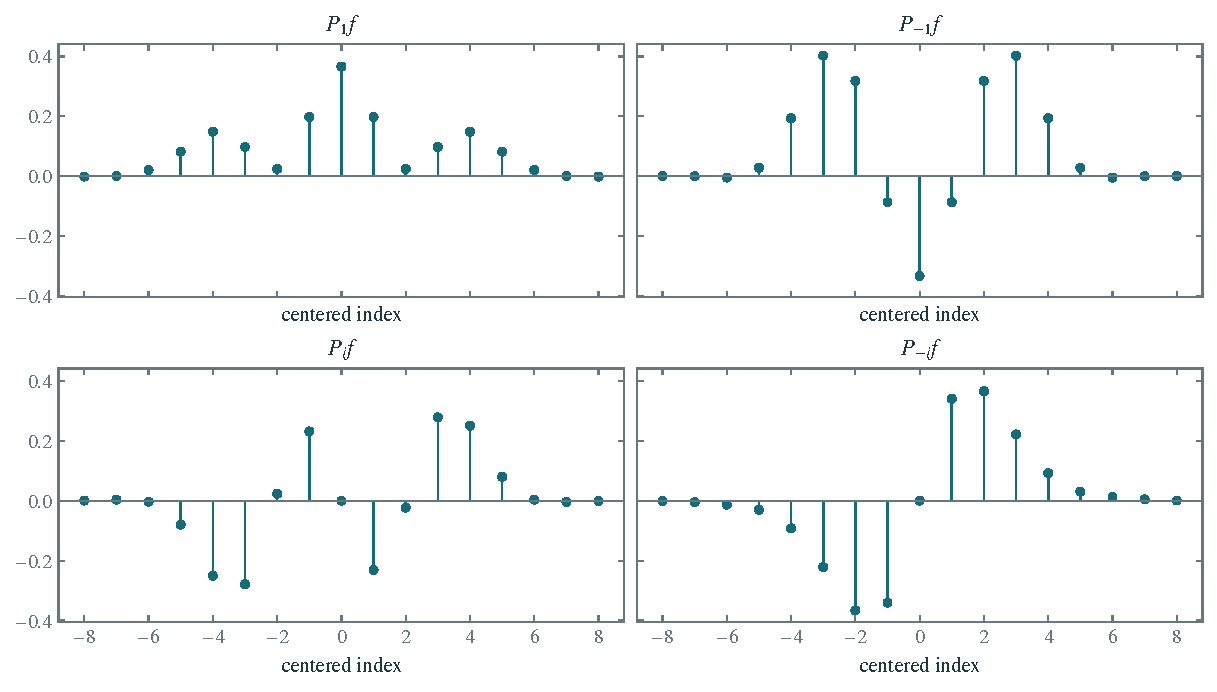
\includegraphics[width=1.0\linewidth]{figures/chapter-discrete-fourier-transform/fourier-eigenspace-projections/figure.pdf}
\caption{The four orthogonal components $P_\lambda f$ of a real signal for the normalized DFT $U$. Their sum is $f$; even and odd components appear on separate rows.}
\label{fig-square-root-tfd}
\end{figure}

To define a consistent family of fractional powers, fix one real phase for
each eigenvalue, for example
\[
 \theta_1=0,\quad\theta_{-1}=\pi,\quad
 \theta_{\imath}=\pi/2,\quad\theta_{-\imath}=-\pi/2.
\]
For every $\alpha\in\RR$, set
\[
 U^\alpha=\sum_{\lambda\in\{1,-1,\imath,-\imath\}}
                   e^{\imath\alpha\theta_\lambda}P_\lambda,
 \qquad \Ff^\alpha=N^{\alpha/2}U^\alpha.
\]
The projector identities give $U^0=I$, $U^1=U$, and
$U^\alpha U^\beta=U^{\alpha+\beta}$; the same composition rule holds for
$\Ff^\alpha$. In particular, $(\Ff^{1/2})^2=\Ff$.
The normalized family preserves norms, whereas
$\norm{\Ff^\alpha f}_2=N^{\alpha/2}\norm f_2$.
The figures use $U^\alpha$ so that changes in shape can be compared at a
fixed energy.
\begin{figure}[tbp]
\centering
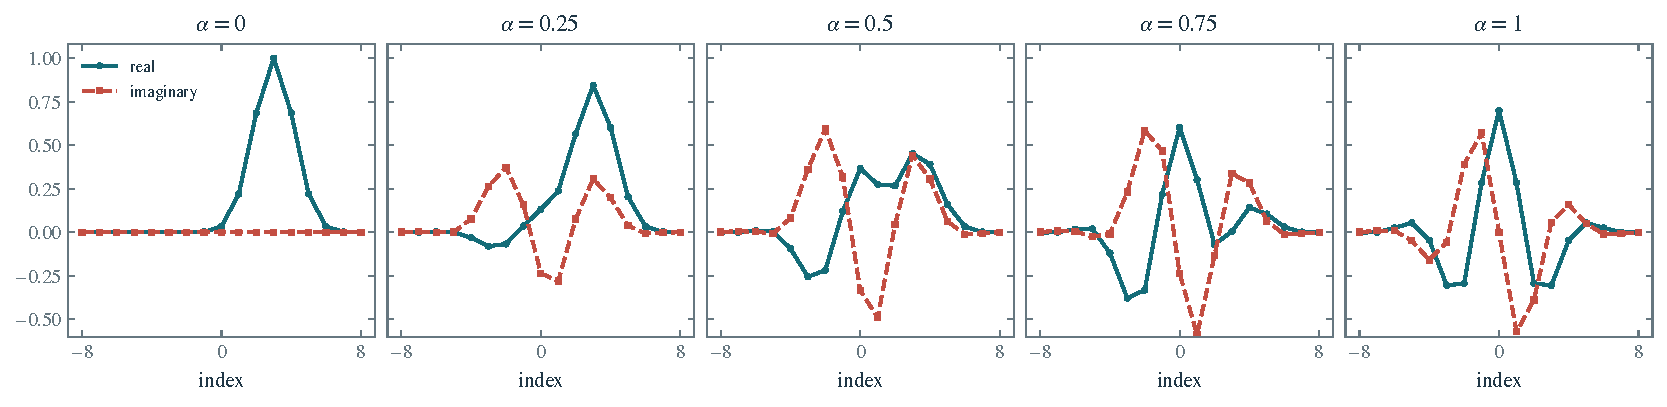
\includegraphics[width=1.0\linewidth]{figures/chapter-discrete-fourier-transform/intermediate-fourier-transform/figure.pdf}
\caption{The unitary transforms $U^\alpha f$ for $0\leq\alpha\leq1$, using the fixed phases in the text. Real and imaginary parts are shown separately.}
\label{fig-root-interm-tfd}
\end{figure}
Choosing other phases modulo $2\pi$ gives other continuous families.
The choices must be fixed for all exponents; choosing a new root independently
at each exponent need not obey the composition law.
Within an eigenspace, changing the orthonormal basis alone has no effect when
its phase is kept the same. Exercise~\ref{exo-transforme-partial-fourier}
explores these choices, while Exercise~\ref{exo-diagonalization-tfd}
constructs a reproducible eigenbasis using a second commuting operator.
For further background see Cariolaro~\cite{cariolaro-partial-fourier}.
\section{Exercises}
\label{sect1-chap2-exercises}

\begin{exo}[Bit reversal]
\label{exo-bit-reversal}\index{Bit reversal}
Define index vectors recursively by
$u^{(0)}=(0)$ and $u^{(n)}=(2u^{(n-1)},2u^{(n-1)}+1)$.
\begin{enumerate}
\item Compute $u^{(n)}$ for $n=1,2,3$.
\item Prove that $u^{(n)}[k]$ reverses the $n$ binary digits of $k$.
\item For a length-$2^n$ vector, let $\wt f[k]=f[u^{(n)}[k]]$.
Explain its role in the iterative DIT algorithm.
\item Show that the first and second halves satisfy
$\wt f_g=\widetilde{f^0}$ and $\wt f_d=\widetilde{f^1}$.
\item Implement this last relation recursively in Python. Compare its array
copying cost with generating $u^{(n)}$ directly by the index-vector recursion.
\end{enumerate}
\end{exo}

\begin{exo}[The Good--Thomas algorithm]
\label{exo-algo-good-thomas}\index{Good--Thomas algorithm}
Let $N=pq$, with $p,q\geq2$ coprime integers. They need not be prime.
\begin{enumerate}
\item Use the Chinese remainder theorem to invert
$\varphi:n\mapsto(n\bmod p,n\bmod q)$ from $\ZZ/N\ZZ$ to
$\ZZ/p\ZZ\times\ZZ/q\ZZ$. Write its inverse as $\psi$.
\item For $F[k_1,k_2]=f[\psi(k_1,k_2)]$, prove
\[
 \wh F[s_1,s_2]=\wh f[(s_1q+s_2p)\bmod N].
\]
\item Show that $(s_1,s_2)\mapsto(s_1q+s_2p)\bmod N$ is a bijection.
Give its inverse explicitly and deduce the output permutation of the algorithm.
\item Explain why this factorization eliminates the twiddle factors in
\eqref{eqn-cooley-tukey-twiddle}. Implement one Good--Thomas step in Python.
Discuss how it can be combined recursively with Cooley--Tukey and with
other algorithms for inconvenient lengths; distinguish arithmetic savings
from the cost of permutations.
\end{enumerate}
\end{exo}

\begin{exo}[The split-radix algorithm]
\label{exo-algo-split-radix}\index{Split-radix FFT}
Let $N=2^p\geq4$. Split-radix keeps the length-$N/2$ transform for the even
frequencies and computes the odd frequencies using two length-$N/4$ transforms.
\begin{enumerate}
\item Starting with a DIF decomposition, prove, for $j=0,1$ and
$0\leq k<N/4$, that
\[
 \wh f[4k+2j+1]=\sum_{a=0}^{N/4-1}\omega_{N/4}^{-ka}\omega_N^{-a(2j+1)}
              \sum_{b=0}^3f[a+bN/4]\omega_4^{-b(2j+1)}.
\]
Express the inner sums using additions, subtractions, and multiplication
by $\pm\imath$. Identify the remaining twiddle factors.
\item Derive the DIT version by separating the input subsequences
$f[2k]$, $f[4k+1]$, and $f[4k+3]$. Give four formulas for the output
quarters and implement the resulting recursion.
\item Compare this recursion with radix two in a specified arithmetic model:
count complex additions and general twiddle multiplications, but regard
multiplication by $\pm\imath$ as a sign change and component swap.
Use direct length-two butterflies as the base case. Count every displayed
twiddle multiplication, even when its factor happens to be one.
Derive recurrences for these counts and compare their leading terms.
Explain what extra work an iterative implementation requires to lay out its
unequal subproblems and permute the data.
\end{enumerate}
The comparison concerns this arithmetic model, not a universal optimality
claim or a guarantee about running time. For further variants see
Vetterli and Nussbaumer~\cite{vetterli-split-radix}.
\end{exo}

\begin{exo}[Overlap-add convolution]
\label{exo-calcul-convolution-fft}\index{Convolution!overlap-add}
Let $f$ and $g$ have lengths $N$ and $M$, with $M\ll N$, and extend both
by zero outside their index intervals starting at zero.
\begin{enumerate}
\item If $N=pM$, let $f_j[k]=f[k+jM]$ for $0\leq k<M$, and extend each
block by zero. Prove
\[
 (f\star g)[k]=\sum_{j=0}^{p-1}(f_j\star g)[k-jM].
\]
\item Compute each block convolution using a common FFT length
$L\geq2M-1$, reuse the transform of $g$, and add the overlapping outputs.
Show that choosing $L=O(M)$ gives total cost $O(N\log M)$ for $M\geq2$.
\item Handle a final block of fewer than $M$ samples when $M\nmid N$.
Implement the method and compare its output with direct linear convolution.
\end{enumerate}
\end{exo}

\begin{exo}[Circulant matrices]
\label{exo-circulating-matrix}\index{Circulant matrix}
For $c\in\CC^N$, let $C_{ij}=c[(i-j)\bmod N]$.
Its first column is $c$, and its first row is $(c_0,c_{N-1},\ldots,c_1)$.
This convention differs from specifying the first row, as in
Exercise~\ref{exo-determinant-circulating}.
\begin{enumerate}
\item Let $R e_j=e_{(j+1)\bmod N}$ for the standard basis indexed from zero.
Prove
\[
 \Omega_NR\Omega_N^{-1}
       =D=\operatorname{diag}(1,\omega_N^{-1},\ldots,\omega_N^{-(N-1)}).
\]
\item Show that $C=\sum_{j=0}^{N-1}c_jR^j$ and deduce
$\Omega_NC\Omega_N^{-1}=\operatorname{diag}(\wh c)$.
Hence show that $Cx=\Omega_N^{-1}((\Omega_Nc)\cdot(\Omega_Nx))$.
\item Verify directly that $Cx=c*x$ for every $x\in\CC^N$.
Recover the diagonalization from the convolution theorem.
\end{enumerate}
\end{exo}

\begin{exo}[Trigonometric interpolation]
\label{exo-interpolation-trigonometric}\index{Trigonometric interpolation}
Let $N=2N_0+1$ be odd and $f\in\CC^N$. Define the trigonometric polynomial
\[
 p(t)=\frac1N\sum_{k=-N_0}^{N_0}\wh f[k\bmod N]e^{2\pi\imath kt}.
\]
For an integer $\eta\geq1$, let $P=\eta N$ and construct the length-$P$
spectrum by inserting zeros between its nonnegative- and negative-frequency
parts:
\[
 \wh{f_0}=\eta\bigl(\wh f[0],\ldots,\wh f[N_0],
                 0,\ldots,0,\wh f[N_0+1],\ldots,\wh f[N-1]\bigr).
\]
Prove that $f_0[j]=p(j/P)$ and $f_0[\eta k]=f[k]$.
Implement the construction for real and complex inputs. Explain why padding
the spectrum must respect the signed frequency indices, and why the factor
$\eta$ is needed. The odd-length assumption avoids a choice for the Nyquist
coefficient that arises at even lengths.
\begin{figure}[tbp]
\centering
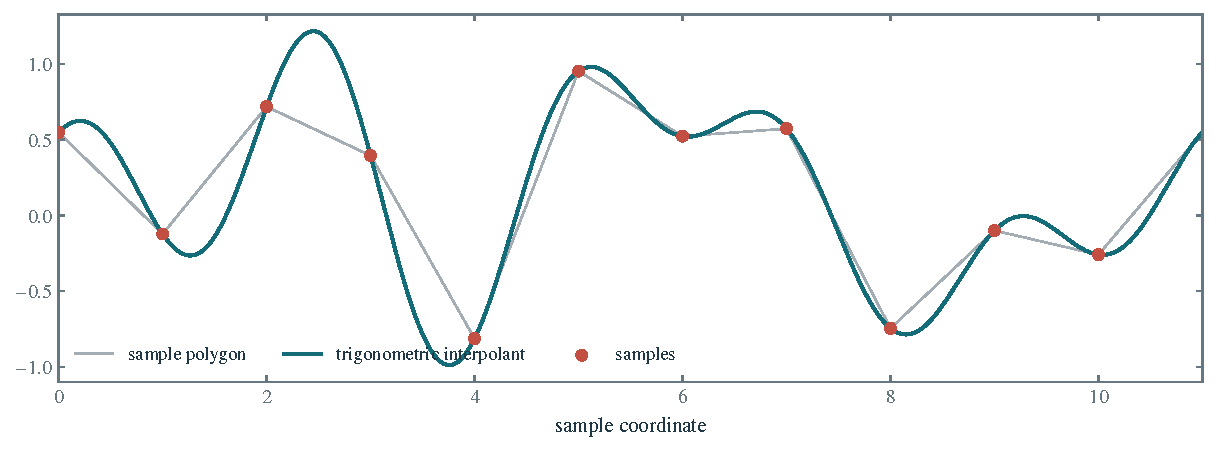
\includegraphics[width=1.0\linewidth]{figures/chapter-discrete-fourier-transform/trigonometric-interpolation/figure.pdf}
\caption{Periodic trigonometric interpolation of eleven samples. The faint polygon joins the samples for reference; it is not an underlying continuous signal.}
\label{fig-fft-interpolation}
\end{figure}
\end{exo}

\begin{exo}[Chebyshev interpolation]
\label{exo-interpolation-chebyshev}\index{Chebyshev polynomials}
For $x\in[-1,1]$, define $T_k(x)=\cos(k\arccos x)$.
\begin{figure}[tbp]
\centering
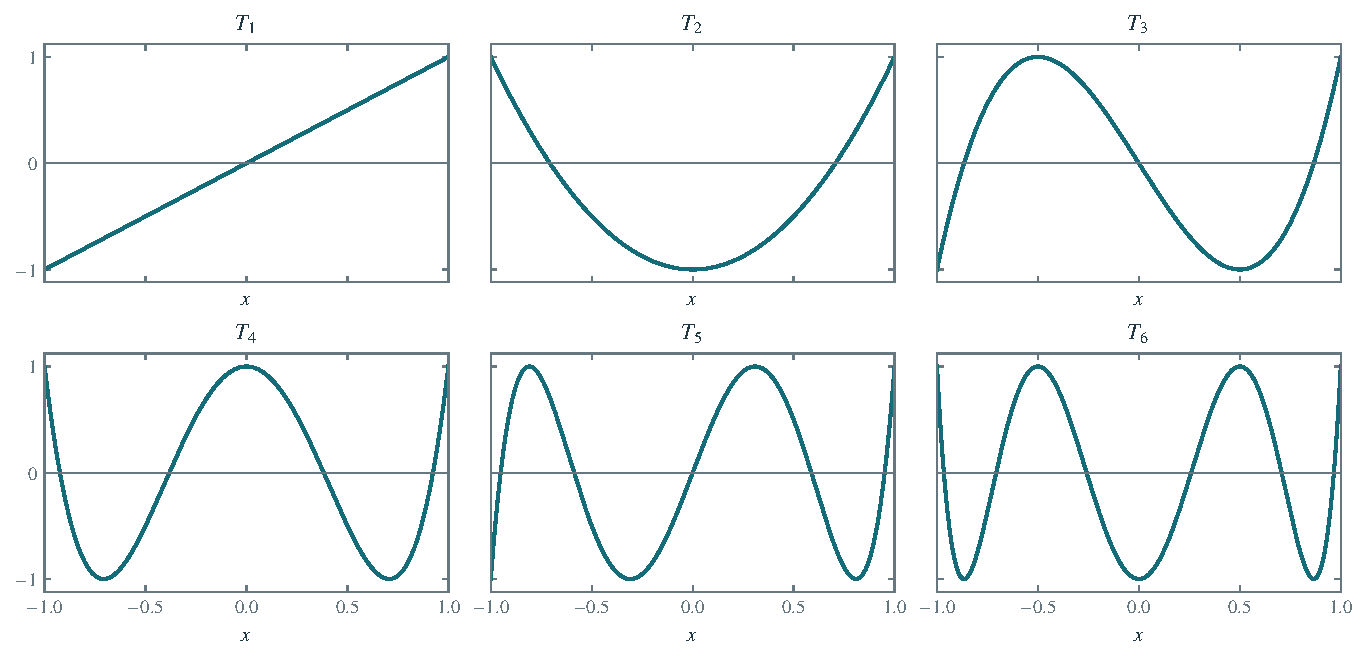
\includegraphics[width=1.0\linewidth]{figures/chapter-discrete-fourier-transform/chebyshev-polynomials/figure.pdf}
\caption{The Chebyshev polynomials $T_k(x)=\cos(k\arccos x)$ for $k=1,\ldots,6$.}
\label{fig-polynomes-chebyshev}
\end{figure}
For $f\in C([-1,1])$, we seek the polynomial of degree at most $N-1$
interpolating $f$ at the Chebyshev nodes
$x_j=\cos((j+1/2)\pi/N)$, $0\leq j<N$.
\begin{enumerate}
\item Prove the recurrence $T_{k+1}=2xT_k-T_{k-1}$, with $T_0=1$ and
$T_1=x$. Deduce that $T_k$ is a polynomial of degree $k$ and that the $x_j$
are exactly the roots of $T_N$.
\item Show that the interpolant has a unique expansion
$P_{N-1}=\sum_{k=0}^{N-1}\alpha_kT_k$.
\item Define the cosine transforms, with the normalization used here, by
\begin{align*}
 \Cc_2(v)[j]&=\sum_{k=0}^{N-1}v[k]\cos((k+1/2)j\pi/N),\\
 \Cc_3(v)[j]&=\tfrac12v[0]+\sum_{k=1}^{N-1}v[k]\cos((j+1/2)k\pi/N).
\end{align*}
Prove that $\Cc_2^{-1}=(2/N)\Cc_3$.
Implement both for real data using a length-$4N$ FFT, specifying the positions
of the inserted zeros. These conventions differ by a factor of two from
SciPy's default unnormalized DCT-II and DCT-III.
\item Express the coefficients $\alpha_k$ in terms of $v[j]=f(x_j)$.
Use the cosine transform to compute them, then evaluate the Chebyshev expansion.
\end{enumerate}
The DCT-II also underlies the block transform used in JPEG; Strang~\cite{strang-dct}
discusses its mathematical structure. Figure~\ref{fig-interpolation-chebyshev}
compares the two node choices for $f(x)=1/(\alpha^2+x^2)$ with $N=11$ and
$\alpha=0.3$. Both interpolants are Lagrange interpolation polynomials;
one uses equally spaced nodes and the other uses Chebyshev nodes.
Explore how their maximum errors change with $N$ and $\alpha$.
A finite plot suggests behavior but does not prove uniform convergence.
\begin{figure}[tbp]
\centering
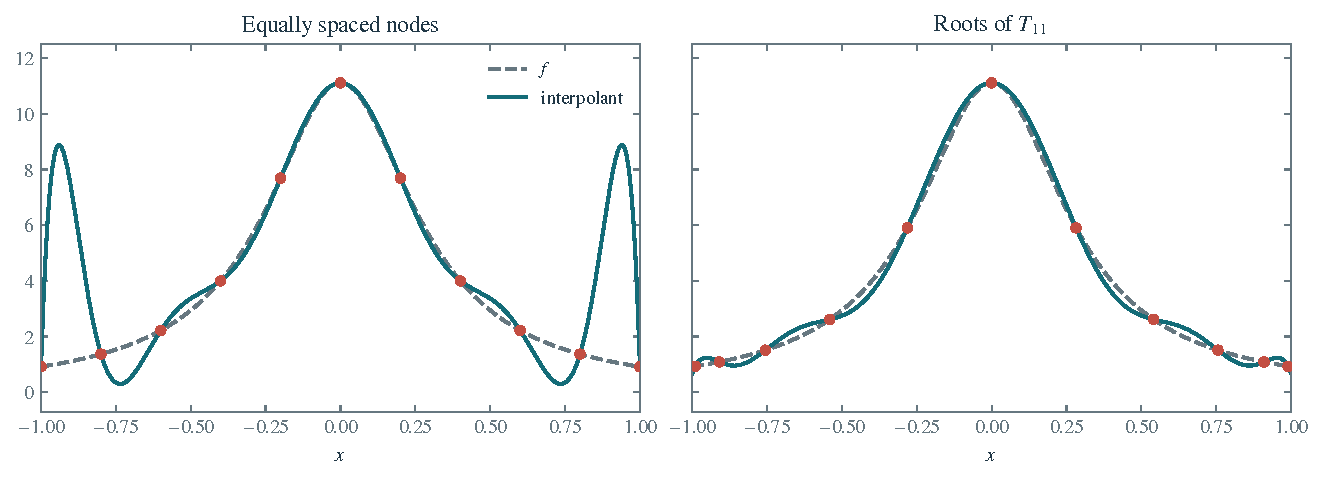
\includegraphics[width=1.0\linewidth]{figures/chapter-discrete-fourier-transform/chebyshev-interpolation/figure.pdf}
\caption{Degree-ten polynomial interpolation of $f(x)=1/(0.3^2+x^2)$ at eleven equally spaced points and at the roots of $T_{11}$. Both are Lagrange interpolants; the choice of nodes controls the endpoint oscillations.}
\label{fig-interpolation-chebyshev}
\end{figure}
Chebyshev expansions are also useful in spectral methods for differential
equations; see Boyd~\cite{boyd-spectral}.
\end{exo}

\begin{exo}[Fractional differentiation]
\label{exo-derivation-fractionionnaire}\index{Fractional differentiation}
Let $f$ be a Schwartz function on $\RR$, with
$\wh f(\xi)=\int f(t)e^{-\imath\xi t}\,\d t$.
Show that $\wh{f^{(m)}}(\xi)=(\imath\xi)^m\wh f(\xi)$ for integers $m\geq0$.
For $\alpha\geq0$, define one fractional derivative by the multiplier
\[
 (\imath\xi)^\alpha=|\xi|^\alpha
             e^{\imath\pi\alpha\operatorname{sgn}(\xi)/2}\quad(\xi\neq0),
\]
setting its value at zero to zero when $\alpha>0$, and to one when $\alpha=0$.
Explain the branch choice and why this operator maps real input to real output.
Implement its periodic discrete analogue on an \emph{odd} number of uniformly
spaced samples over a specified period. Compare integer orders with known
derivatives and discuss periodization and sampling errors when using it to
approximate differentiation on $\RR$.
\begin{figure}[tbp]
\centering
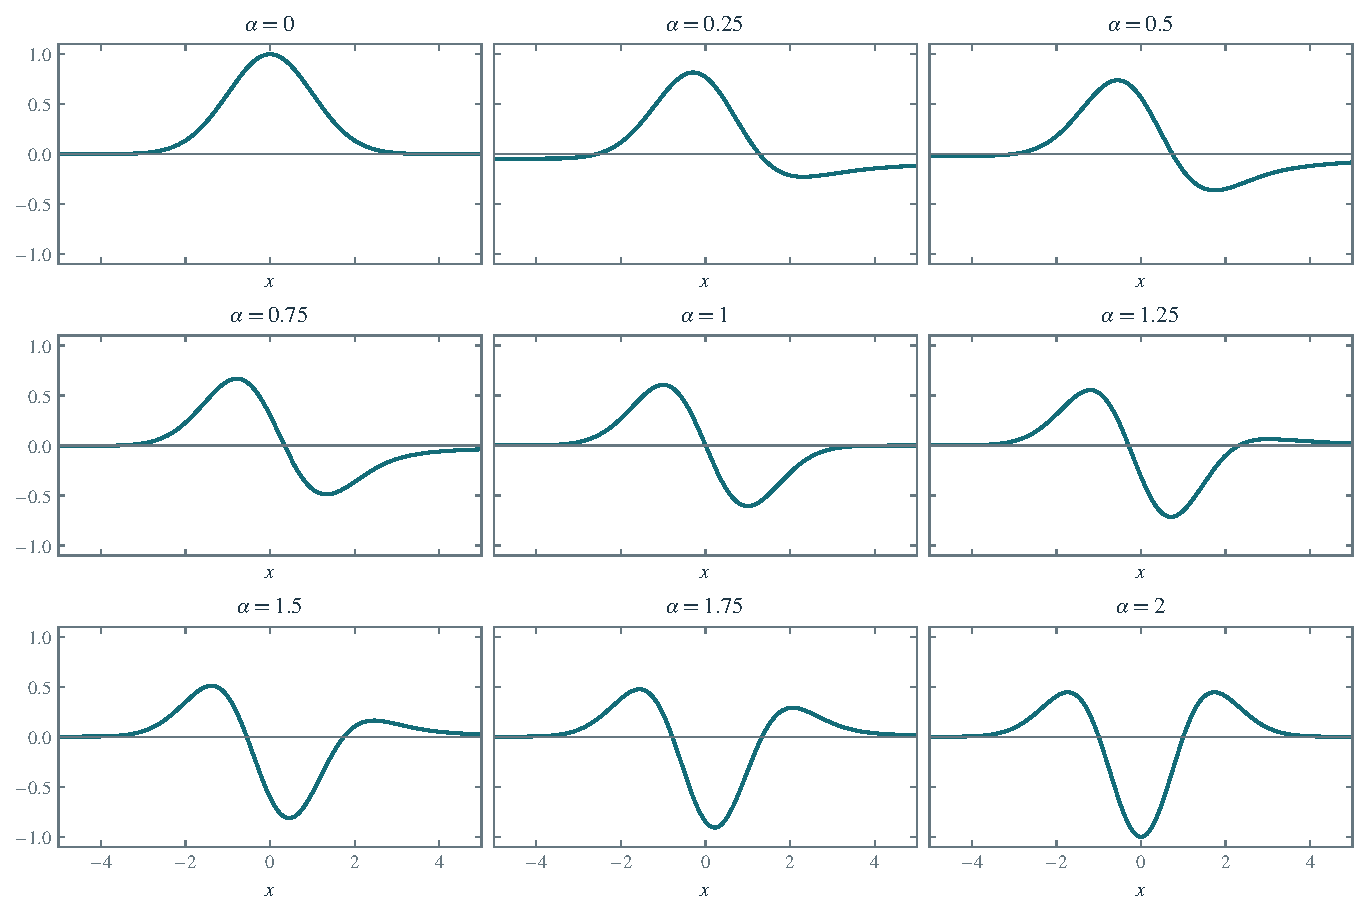
\includegraphics[width=1.0\linewidth]{figures/chapter-discrete-fourier-transform/fractional-differentiation/figure.pdf}
\caption{Fractional derivatives of $e^{-x^2/2}$ for orders $0\leq\alpha\leq2$, computed from the multiplier $(\imath\xi)^\alpha$ with the phase convention in the text.}
\label{fig-derivation-fractionionnaire}
\end{figure}
\end{exo}

\begin{exo}[Intermediate Fourier transforms]
\label{exo-transforme-partial-fourier}\index{Fractional Fourier transform!discrete}
Let $U=\Omega_N/\sqrt N$ be the unitary DFT.
\begin{enumerate}
\item Prove that $U$ is normal and $U^4=I$. List the possible eigenvalues,
and explain why normality, rather than a false Hermitian assumption, gives
an orthonormal eigenbasis.
\item Let $P_\lambda$ be its spectral projectors. Fix phases
$e^{\imath\theta_\lambda}=\lambda$ and define
$U^\alpha=\sum_\lambda e^{\imath\alpha\theta_\lambda}P_\lambda$.
Prove $U^\alpha U^\beta=U^{\alpha+\beta}$, $U^1=U$, and unitarity.
Why must the phases be chosen consistently for all exponents?
\item Show that $U^2$ is cyclic reversal and explain the identity and reversal
diagonals visible in Figure~\ref{fig-matrix-partial-tfd}.
Give the corresponding formulas for the unnormalized $\Omega_N^\alpha$.
\begin{figure}[tbp]
\centering
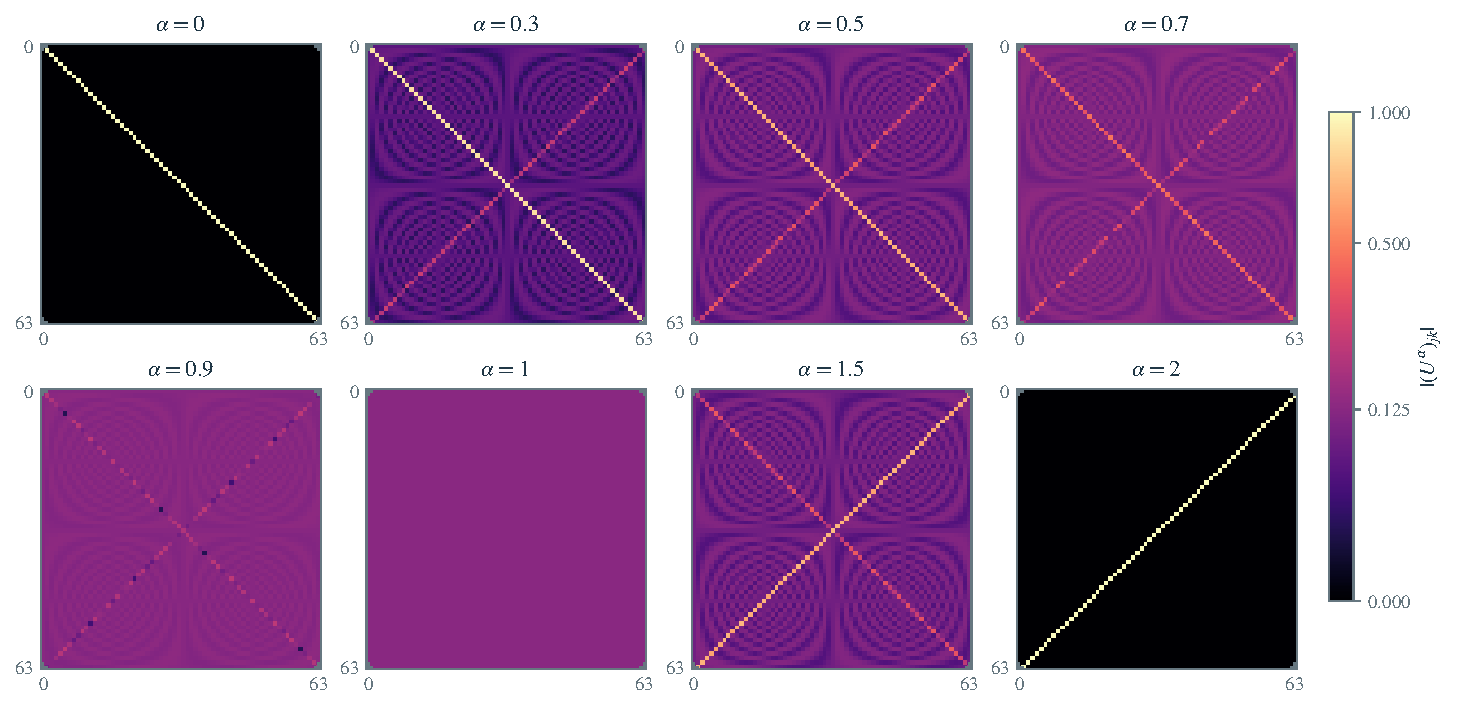
\includegraphics[width=1.0\linewidth]{figures/chapter-discrete-fourier-transform/fractional-fourier-matrices/figure.pdf}
\caption{Entrywise magnitudes of the unitary matrices $U^\alpha$, on one common nonlinear color scale. At $\alpha=1$ every magnitude equals $1/\sqrt N$; at $\alpha=2$ the matrix is cyclic reversal.}
\label{fig-matrix-partial-tfd}
\end{figure}
\item Explain why changing a basis inside an eigenspace leaves the result
unchanged when the phase is fixed for that whole eigenspace.
Construct distinct families by changing a phase by an integer multiple of
$2\pi$, and implement the transform using the explicit projectors.
Check the composition law numerically for noninteger exponents.
\end{enumerate}
Figure~\ref{fig-transforme-partial-fourier} uses the phases fixed in
Section~\ref{sect2-eigenvalues-tfd}. A symmetric input returns to itself at
$\alpha=2$ under this normalized transform. The unnormalized transform
would return $N$ times that input.
\begin{figure}[tbp]
\centering
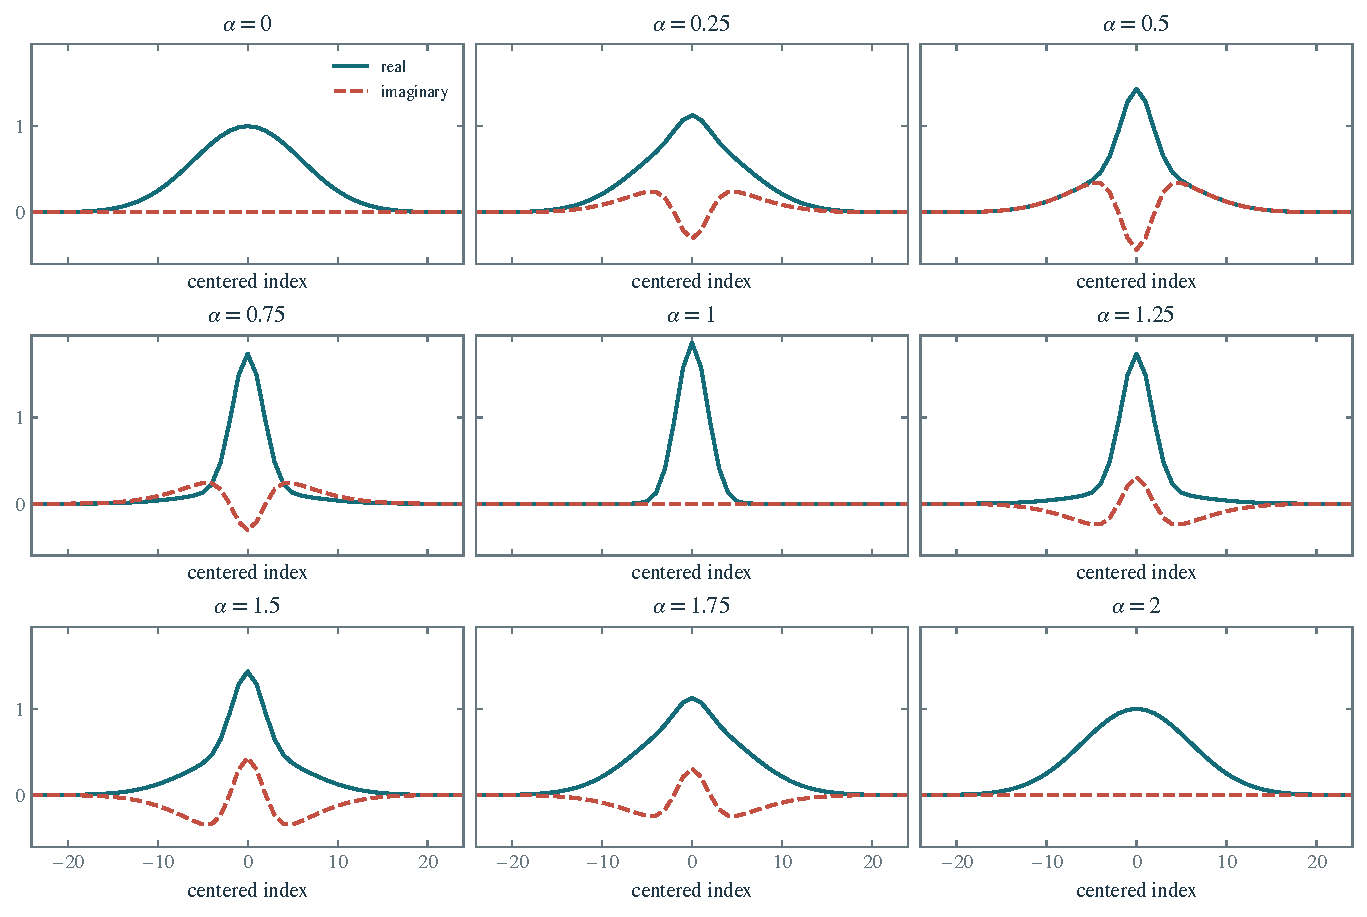
\includegraphics[width=1.0\linewidth]{figures/chapter-discrete-fourier-transform/fractional-fourier-gaussian/figure.pdf}
\caption{Unitary fractional Fourier transforms of a discrete Gaussian. The fixed eigenspace phases give a continuous family; at $\alpha=2$ this even input is recovered.}
\label{fig-transforme-partial-fourier}
\end{figure}
\end{exo}

\begin{exo}[A structured eigenbasis of the DFT]
\label{exo-diagonalization-tfd}\label{notation-50}\label{notation-51}
\index{Fourier matrix!eigenvectors}
For $N\geq3$, let $R e_j=e_{j+1\bmod N}$ and define the real symmetric matrix
\[
 S=R+R^{\mathsf T}
       +\operatorname{diag}\bigl(2\cos(2\pi k/N)-4\bigr)_{k=0}^{N-1}.
\]
The construction is based on Dickinson and Steiglitz~\cite{dickinson-eigenvectors};
Candan, Kutay, and Ozaktas~\cite{candan-fractional} relate such eigenvectors
to discrete fractional transforms.
\begin{enumerate}
\item Explain why $S$ admits a real orthonormal eigenbasis.
\item Set $\Gamma=R+R^{\mathsf T}-2I$ and
$\Delta=\operatorname{diag}(2\cos(2\pi k/N)-2)$.
Prove $\Omega_N\Gamma=\Delta\Omega_N$ and
$\Omega_N\Delta=\Gamma\Omega_N$, and conclude that $S$ commutes with $\Omega_N$.
\item Prove that commuting diagonalizable operators on $\CC^N$ have a common
eigenbasis. Explain why common eigenspaces need further care if an eigenvalue
of one operator is repeated.
\item Restrict $S$ to the symmetric and antisymmetric subspaces for cyclic
reversal. Use the symmetric basis $e_0$,
$(e_k+e_{N-k})/\sqrt2$ for $1\leq k<N/2$, and also $e_{N/2}$ if $N$ is even;
use $(e_k-e_{N-k})/\sqrt2$ for the antisymmetric basis.
Show that each restriction is a real symmetric tridiagonal matrix with every
subdiagonal entry nonzero, except when its dimension is one.
\item Prove that each such tridiagonal matrix has distinct eigenvalues by
showing that an eigenvector is determined by its first coordinate.
Explain why this conclusion applies separately to the two parity blocks,
and does not imply that all eigenvalues of $S$ are distinct.
Check that $S$ has the repeated eigenvalue $-4$ when $N=4$.
\item Deduce that diagonalizing each parity block yields common eigenvectors
of $S$ and $\Omega_N$, including when their eigenvalues of $S$ overlap.
Choose an ordering and signs to make the numerical output reproducible,
and check the eigenvector residuals and orthogonality.
\end{enumerate}
The figures use decreasing eigenvalue of $S$, with a specified tie convention.
This makes the construction reproducible; it does not remove the freedom
inherent in choosing an additional commuting operator and an ordering.
\begin{figure}[tbp]
\centering
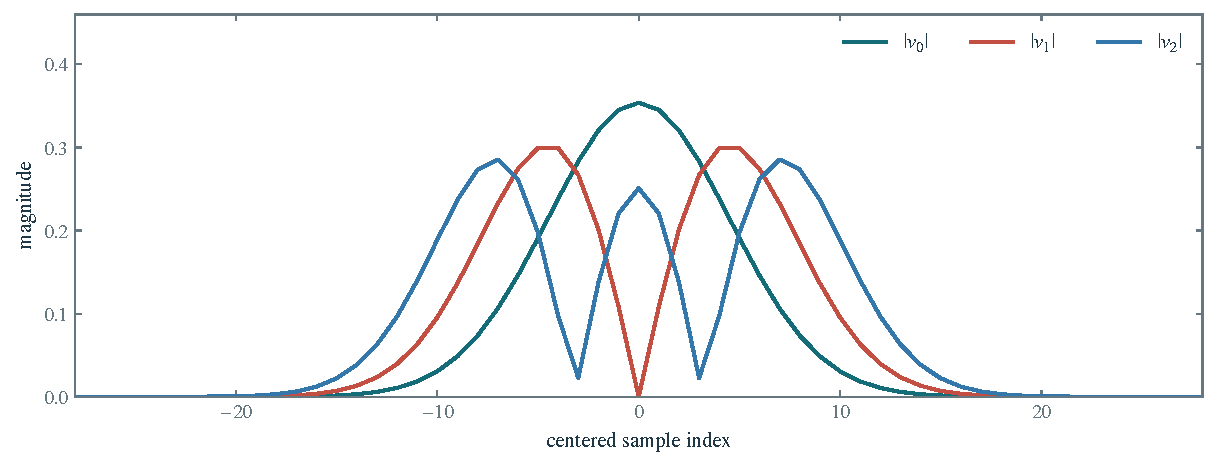
\includegraphics[width=1.0\linewidth]{figures/chapter-discrete-fourier-transform/fourier-eigenvectors/figure.pdf}
\caption{Magnitudes of the first three vectors in the structured DFT eigenbasis for $N=128$, ordered by decreasing eigenvalue of $S$. The index is centered for display.}
\label{fig-eigenvectors-tfd}
\end{figure}
\begin{figure}[tbp]
\centering
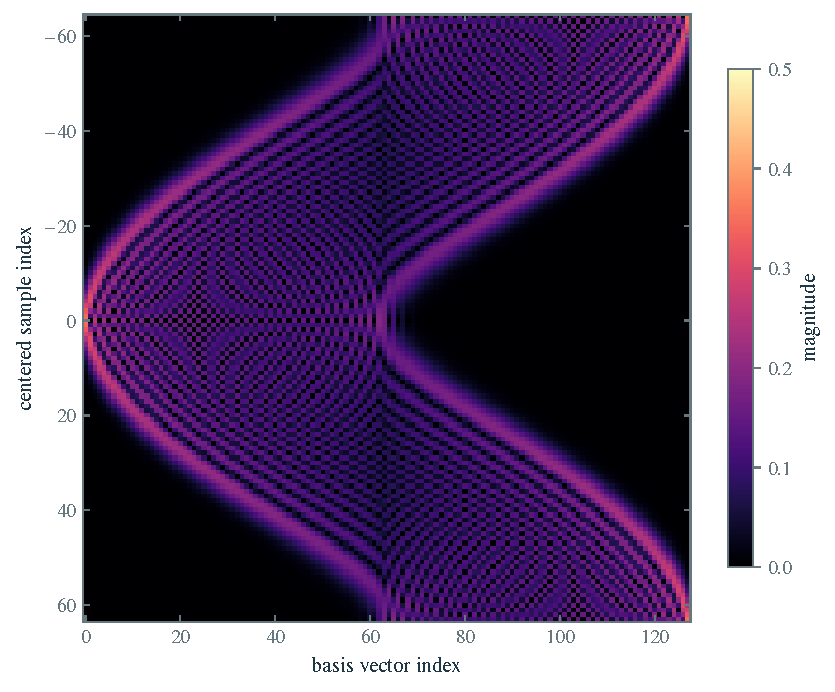
\includegraphics[width=.64\linewidth]{figures/chapter-discrete-fourier-transform/fourier-eigenbasis-matrix/figure.pdf}
\caption{Magnitudes of the structured orthonormal eigenbasis for $N=128$. Columns follow decreasing eigenvalues of $S$, with even parity first in a tie; rows show centered sample indices.}
\label{fig-matrix-eigenvectors-tfd}
\end{figure}
\end{exo}

\begin{exo}[Orthogonalizing cyclic translates]
\label{exo-orthogonalization-fourier}\index{Orthogonalization}
On $G=\ZZ/n\ZZ$, use the normalized inner product
$\dotp fg=n^{-1}\sum_xf[x]\ol{g[x]}$.
Define translation and modulation by
\[
 (k\top f)[x]=f[x-k],\qquad (k\bot f)[x]=\omega_n^{-kx}f[x].
\]
All indices are taken modulo $n$.
\begin{enumerate}
\item Prove
$\Ff(k\top f)=k\bot\Ff(f)$ and
$\Ff(k\bot f)=(-k)\top\Ff(f)$.
\item Explain how the \emph{unitary} transform $n^{-1/2}\Ff$ maps an
orthonormal translation orbit to an orthonormal modulation orbit, and conversely.
\item Show that $\{k\top f\}_{k\in G}$ is orthonormal if and only if
$|\wh f[k]|=\sqrt n$ for every $k$.
\item When $\wh f$ has no zero entry, define
$\wh{f_0}[k]=\sqrt n\,\wh f[k]/|\wh f[k]|$.
Show that the translates of $f_0$ are orthonormal.
Give the analogous pointwise normalization for a modulation orbit, assuming
$f[x]\neq0$ everywhere.
\item If the translates of $g$ are orthonormal, express
$\Gg(\varphi)[k]=\dotp\varphi{k\top g}$ as a circular correlation:
\[
 \Gg(\varphi)=\frac1n\varphi*\wt g,
 \qquad \wt g[x]=\ol{g[-x]}.
\]
Deduce an $O(n\log n)$ coefficient algorithm and the reconstruction of
$\varphi$ from these coefficients.
\end{enumerate}
Figure~\ref{fig-orthogonalisation-fourier} shows how replacing Fourier
magnitudes by the constant $\sqrt n$ changes the signal.
The effect depends on its spectral phases; it is not a universal increase
in oscillation or a smoothing operation.
\begin{figure}[tbp]
\centering
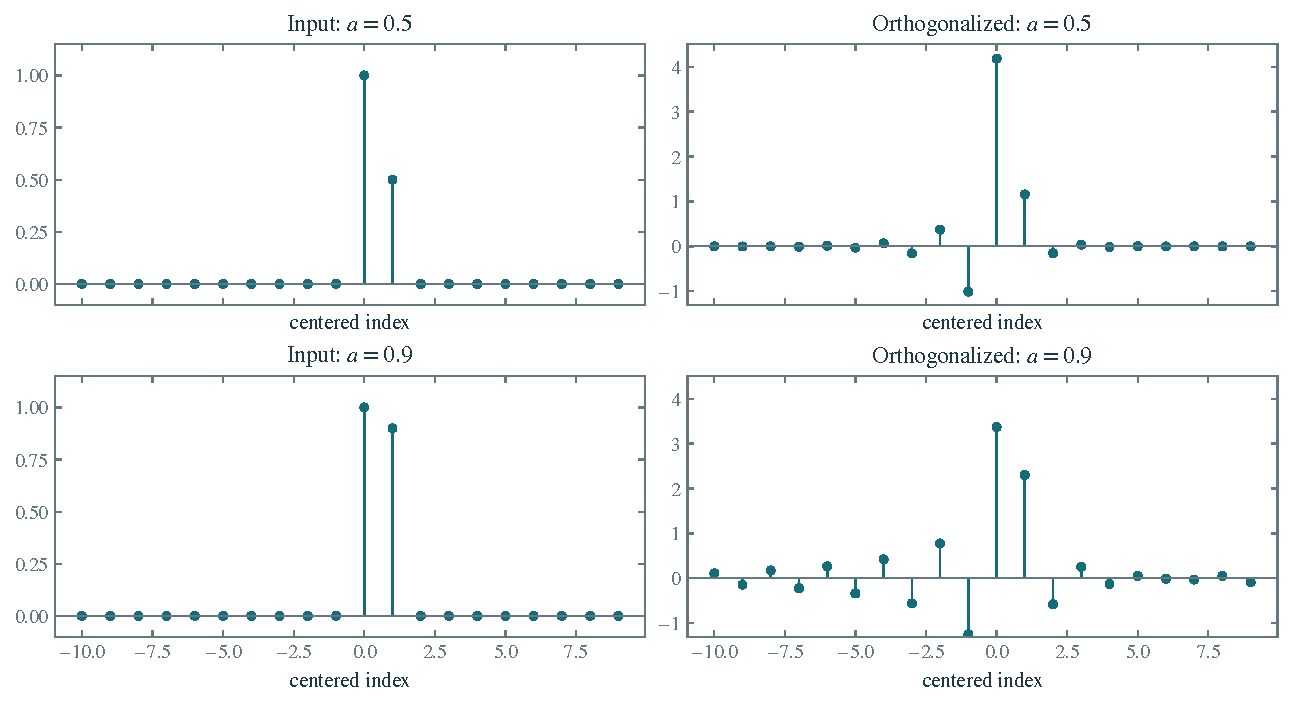
\includegraphics[width=1.0\linewidth]{figures/chapter-discrete-fourier-transform/orthogonalizing-translates/figure.pdf}
\caption{Orthogonalizing the cyclic translates of $f=\delta_0+a\delta_1$ on $\ZZ/20\ZZ$, for $a=0.5$ and $a=0.9$. The output $g$ satisfies $|\widehat g|=\sqrt{20}$, as required by the normalized inner product.}
\label{fig-orthogonalisation-fourier}
\end{figure}
\end{exo}
